% Options for packages loaded elsewhere
% Options for packages loaded elsewhere
\PassOptionsToPackage{unicode}{hyperref}
\PassOptionsToPackage{hyphens}{url}
\PassOptionsToPackage{dvipsnames,svgnames,x11names}{xcolor}
%
\documentclass[
  11pt,
  letterpaper,
  DIV=11,
  numbers=noendperiod]{scrartcl}
\usepackage{xcolor}
\usepackage[margin=1.1in]{geometry}
\usepackage{amsmath,amssymb}
\setcounter{secnumdepth}{5}
\usepackage{iftex}
\ifPDFTeX
  \usepackage[T1]{fontenc}
  \usepackage[utf8]{inputenc}
  \usepackage{textcomp} % provide euro and other symbols
\else % if luatex or xetex
  \usepackage{unicode-math} % this also loads fontspec
  \defaultfontfeatures{Scale=MatchLowercase}
  \defaultfontfeatures[\rmfamily]{Ligatures=TeX,Scale=1}
\fi
\usepackage{lmodern}
\ifPDFTeX\else
  % xetex/luatex font selection
\fi
% Use upquote if available, for straight quotes in verbatim environments
\IfFileExists{upquote.sty}{\usepackage{upquote}}{}
\IfFileExists{microtype.sty}{% use microtype if available
  \usepackage[]{microtype}
  \UseMicrotypeSet[protrusion]{basicmath} % disable protrusion for tt fonts
}{}
\makeatletter
\@ifundefined{KOMAClassName}{% if non-KOMA class
  \IfFileExists{parskip.sty}{%
    \usepackage{parskip}
  }{% else
    \setlength{\parindent}{0pt}
    \setlength{\parskip}{6pt plus 2pt minus 1pt}}
}{% if KOMA class
  \KOMAoptions{parskip=half}}
\makeatother
% Make \paragraph and \subparagraph free-standing
\makeatletter
\ifx\paragraph\undefined\else
  \let\oldparagraph\paragraph
  \renewcommand{\paragraph}{
    \@ifstar
      \xxxParagraphStar
      \xxxParagraphNoStar
  }
  \newcommand{\xxxParagraphStar}[1]{\oldparagraph*{#1}\mbox{}}
  \newcommand{\xxxParagraphNoStar}[1]{\oldparagraph{#1}\mbox{}}
\fi
\ifx\subparagraph\undefined\else
  \let\oldsubparagraph\subparagraph
  \renewcommand{\subparagraph}{
    \@ifstar
      \xxxSubParagraphStar
      \xxxSubParagraphNoStar
  }
  \newcommand{\xxxSubParagraphStar}[1]{\oldsubparagraph*{#1}\mbox{}}
  \newcommand{\xxxSubParagraphNoStar}[1]{\oldsubparagraph{#1}\mbox{}}
\fi
\makeatother


\usepackage{longtable,booktabs,array}
\newcounter{none} % for unnumbered tables
\usepackage{calc} % for calculating minipage widths
% Correct order of tables after \paragraph or \subparagraph
\usepackage{etoolbox}
\makeatletter
\patchcmd\longtable{\par}{\if@noskipsec\mbox{}\fi\par}{}{}
\makeatother
% Allow footnotes in longtable head/foot
\IfFileExists{footnotehyper.sty}{\usepackage{footnotehyper}}{\usepackage{footnote}}
\makesavenoteenv{longtable}
\usepackage{graphicx}
\makeatletter
\newsavebox\pandoc@box
\newcommand*\pandocbounded[1]{% scales image to fit in text height/width
  \sbox\pandoc@box{#1}%
  \Gscale@div\@tempa{\textheight}{\dimexpr\ht\pandoc@box+\dp\pandoc@box\relax}%
  \Gscale@div\@tempb{\linewidth}{\wd\pandoc@box}%
  \ifdim\@tempb\p@<\@tempa\p@\let\@tempa\@tempb\fi% select the smaller of both
  \ifdim\@tempa\p@<\p@\scalebox{\@tempa}{\usebox\pandoc@box}%
  \else\usebox{\pandoc@box}%
  \fi%
}
% Set default figure placement to htbp
\def\fps@figure{htbp}
\makeatother


% definitions for citeproc citations
\NewDocumentCommand\citeproctext{}{}
\NewDocumentCommand\citeproc{mm}{%
  \begingroup\def\citeproctext{#2}\cite{#1}\endgroup}
\makeatletter
 % allow citations to break across lines
 \let\@cite@ofmt\@firstofone
 % avoid brackets around text for \cite:
 \def\@biblabel#1{}
 \def\@cite#1#2{{#1\if@tempswa , #2\fi}}
\makeatother
\newlength{\cslhangindent}
\setlength{\cslhangindent}{1.5em}
\newlength{\csllabelwidth}
\setlength{\csllabelwidth}{3em}
\newenvironment{CSLReferences}[2] % #1 hanging-indent, #2 entry-spacing
 {\begin{list}{}{%
  \setlength{\itemindent}{0pt}
  \setlength{\leftmargin}{0pt}
  \setlength{\parsep}{0pt}
  % turn on hanging indent if param 1 is 1
  \ifodd #1
   \setlength{\leftmargin}{\cslhangindent}
   \setlength{\itemindent}{-1\cslhangindent}
  \fi
  % set entry spacing
  \setlength{\itemsep}{#2\baselineskip}}}
 {\end{list}}
\usepackage{calc}
\newcommand{\CSLBlock}[1]{\hfill\break\parbox[t]{\linewidth}{\strut\ignorespaces#1\strut}}
\newcommand{\CSLLeftMargin}[1]{\parbox[t]{\csllabelwidth}{\strut#1\strut}}
\newcommand{\CSLRightInline}[1]{\parbox[t]{\linewidth - \csllabelwidth}{\strut#1\strut}}
\newcommand{\CSLIndent}[1]{\hspace{\cslhangindent}#1}



\setlength{\emergencystretch}{3em} % prevent overfull lines

\providecommand{\tightlist}{%
  \setlength{\itemsep}{0pt}\setlength{\parskip}{0pt}}



 


\KOMAoption{captions}{tableheading}
\usepackage{tgpagella}
\usepackage[scaled=0.94]{helvet}
\makeatletter
\@ifpackageloaded{caption}{}{\usepackage{caption}}
\AtBeginDocument{%
\ifdefined\contentsname
  \renewcommand*\contentsname{Table of contents}
\else
  \newcommand\contentsname{Table of contents}
\fi
\ifdefined\listfigurename
  \renewcommand*\listfigurename{List of Figures}
\else
  \newcommand\listfigurename{List of Figures}
\fi
\ifdefined\listtablename
  \renewcommand*\listtablename{List of Tables}
\else
  \newcommand\listtablename{List of Tables}
\fi
\ifdefined\figurename
  \renewcommand*\figurename{Figure}
\else
  \newcommand\figurename{Figure}
\fi
\ifdefined\tablename
  \renewcommand*\tablename{Table}
\else
  \newcommand\tablename{Table}
\fi
}
\@ifpackageloaded{float}{}{\usepackage{float}}
\floatstyle{ruled}
\@ifundefined{c@chapter}{\newfloat{codelisting}{h}{lop}}{\newfloat{codelisting}{h}{lop}[chapter]}
\floatname{codelisting}{Listing}
\newcommand*\listoflistings{\listof{codelisting}{List of Listings}}
\makeatother
\makeatletter
\makeatother
\makeatletter
\@ifpackageloaded{caption}{}{\usepackage{caption}}
\@ifpackageloaded{subcaption}{}{\usepackage{subcaption}}
\makeatother
\usepackage{bookmark}
\IfFileExists{xurl.sty}{\usepackage{xurl}}{} % add URL line breaks if available
\urlstyle{same}
\hypersetup{
  pdftitle={MacKenzie Scott's giving{,} in QALYs},
  pdfauthor={Max Ghenis},
  colorlinks=true,
  linkcolor={blue},
  filecolor={Maroon},
  citecolor={Blue},
  urlcolor={Blue},
  pdfcreator={LaTeX via pandoc}}


\title{MacKenzie Scott's giving, in QALYs}
\usepackage{etoolbox}
\makeatletter
\providecommand{\subtitle}[1]{% add subtitle to \maketitle
  \apptocmd{\@title}{\par {\large #1 \par}}{}{}
}
\makeatother
\subtitle{An evidence-weighted, auditable cost-effectiveness model of a
\$26 billion portfolio}
\author{Max
Ghenis\thanks{max@maxghenis.com. I am CEO of PolicyEngine and president of the Axiom Foundation; this paper is a personal research project and does not represent the views of either organization. Interactive version, code, data, and full audit trail: \url{https://maxghenis.com/mackenzie-scott-qaly} and \url{https://github.com/MaxGhenis/mackenzie-scott-qaly}.}}
\date{}
\begin{document}
\maketitle
\begin{abstract}
MacKenzie Scott has disclosed \$26.39 billion in gifts to more than
2,500 organizations since 2019 --- roughly a third of American
megagiving in 2025 --- yet almost none of it is denominated in outcomes.
This paper prices the entire portfolio in quality-adjusted life-years. A
Monte Carlo model allocates dollars across 14 intervention archetypes
using Scott's own gift-level database, imputes the undisclosed third
from recipients' pre-gift IRS 990 revenue, assigns each archetype a
cost-per-QALY anchor from published causal estimates, and shrinks every
effect toward zero in proportion to the causal credibility of its
evidence. The best-guess estimate is a median of roughly 202,000 QALYs
(90\% interval 94,000--419,000), a blended \$150,000 per QALY, and a
benefit--cost ratio of 4.9 at the U.S. government's value per QALY.
Three findings follow. First, impact is geographically concentrated: the
4.8\% of dollars funding health and development delivered outside the
United States produces 69\% of estimated health impact. Second, gift
size scales with recipient size to only the 0.41 power --- a 10× larger
organization receives about 2.5× more money. Third, the answer is
dominated by evidence philosophy rather than arithmetic: restricting to
randomized evidence collapses the median to \textasciitilde9,000 QALYs
while taking every study at face value raises it to
\textasciitilde415,000, a 45× range that dwarfs every other modeling
choice. All parameters, code, data snapshots, and an AI-audit trail are
public, and the model runs interactively in the browser.
\end{abstract}


\textsubscript{Source:
\href{https://MaxGhenis.github.io/mackenzie-scott-qaly/index.qmd.html}{Article
Notebook}}

\section{Introduction}\label{introduction}

MacKenzie Scott gave away \$7 billion in 2025 --- by the Indiana
University Lilly Family School of Philanthropy's accounting, about a
third of every megagift in America that year (Indiana University Lilly
Family School of Philanthropy 2026; Konish 2025). Her disclosed lifetime
total is \$26.39 billion across 2,711 gifts to 2,545 organizations since
2019 (Yield Giving 2026). Almost none of it is denominated in health,
and no published estimate prices the portfolio in outcomes of any kind.

This paper does so in the unit health economists use to compare a death
averted against years lived in better health: the quality-adjusted
life-year. The exercise is deliberately in the style of a charity
evaluator's cost-effectiveness analysis (GiveWell 2026), scaled from a
program to a portfolio, with one addition the setting forces: because
most of the portfolio funds interventions whose health effects have
never been causally measured, the model makes its epistemics explicit.
Every effect is shrunk toward zero in proportion to how well its
supporting study identifies causation, the shrinkage schedule is a
slider rather than a buried constant, and the headline is reported
across the full range of evidence philosophies --- from counting only
randomized evidence to taking every published estimate at face value.

The paper makes four contributions. It provides, to my knowledge, the
first portfolio-level cost-effectiveness estimate for a major
philanthropist: a best-guess median of 202,000 QALYs from \$26.39
billion nominal (\$30.3B in 2026 dollars), a blended \$150,067 per QALY,
and a benefit--cost ratio of 4.9 at the U.S. government's value per QALY
(U.S. Department of Health and Human Services, Office of the Assistant
Secretary for Planning and Evaluation 2026). It documents extreme
geographic concentration of modeled impact: the 4.8\% of dollars funding
global health and development delivered outside the United States
accounts for 69.1\% of estimated health impact. It reports a new
empirical regularity in the gift data itself: across 1,313 disclosed
gift--filing pairs, gift size scales with recipient pre-gift revenue to
the power 0.41 (R² 0.37) --- Scott's giving is far flatter across
organization size than proportional. And it demonstrates a working
method for auditable, AI-assisted cost-effectiveness modeling: the model
was built with a frontier language model, reviewed and corrected in
public across eleven revision rounds, audited by two independent model
families against primary filings, and ships with versioned parameters,
machine-checked citations, and a browser implementation that reruns the
full Monte Carlo under any reader's assumptions.

The unit of account deserves a caveat before any number. QALYs measure
health. Most of Scott's portfolio aims at other things --- education,
economic mobility, equity, civic infrastructure --- whose primary
benefits are not health benefits. A finding that a dollar of education
philanthropy produces few QALYs is a statement about the lens, not a
verdict on the gift. The estimates here are a lower bound on total
wellbeing produced, measured along the one dimension with a mature
comparative literature.

\section{Data}\label{data}

\subsection{The ledger}\label{the-ledger}

Scott's essays disclose giving in dated tranches totaling \$26.39
billion nominal over 2020--2025. The model inflates each tranche to 2026
dollars with CPI-U, so dollars and cost-effectiveness evidence share one
price level: \$30.3B total. All derivations below, and the replication
repository, start from a verbatim snapshot of the Yield Giving gift
database retrieved July 11, 2026 (Yield Giving 2026).

\subsection{Allocation across causes}\label{allocation-across-causes}

Scott publishes no aggregate dollars-by-cause breakdown, but she
publishes better: a gift-level database listing every recipient
organization, its self-reported focus areas, and --- for 2,035 of 2,711
gifts (\$17.46B, about two-thirds of the nominal total) --- the dollar
amount. Each organization's dollars are split equally across its focus
areas; the database's 53 areas map onto the model's 14 intervention
archetypes under a documented, sync-tested crosswalk.

The undisclosed third is imputed rather than dropped. Because the essays
give each year's total, the undisclosed residual per period is a known
dollar amount; it is distributed across that period's undisclosed gifts
in proportion to each recipient's pre-gift IRS Form 990 total revenue
(ProPublica 2026), raised to an elasticity fit on the disclosed pairs.
Pre-gift means the latest filing strictly before the gift year, since a
Scott gift mechanically inflates receipt-year revenue. The fit is a
finding in its own right: across 1,313 disclosed gift--filing pairs, log
gift size rises with log revenue with slope 0.41 (R² 0.37). A 10× larger
organization receives about 2.5× more money, not 10× more. Fuzzy
name-to-EIN matches were audited by a third, smaller model against the
live IRS API, with corrections committed as a reviewable overlay. The
imputed third moves each cause share by at most about 1.5 percentage
points --- the disclosed two-thirds is representative.

\subsection{Delivery geography}\label{delivery-geography}

Each organization reports service locations. Weighting disclosed dollars
by the share of an organization's locations outside the United States,
an estimated 20\% of disclosed dollars (\$3.57 billion of \$17.46B) goes
to organizations serving abroad, led by environment, health, and funding
intermediaries. The model prices geography through a single channel:
health-relevant dollars route to a global-health archetype in proportion
to the recipient's non-U.S. service share, because global health
delivery is the one category with a published cost-per-QALY evidence
base an order of magnitude below U.S. anchors. Education and climate
dollars keep their U.S.-study anchors wherever they are delivered; if
geography changes their effectiveness, the model does not capture it.

The coarsest geographic field is the bare label ``global.'' An audit of
the 50 largest organizations reporting only that label --- 87\% of that
bucket's dollars --- replaced the blanket assumption of fully-abroad
delivery with fractions taken from each organization's own filings and
program reports, independently verified by a second model family, with
per-organization sources committed to the repository. Many ``global''
organizations operate substantially in the United States: Planned
Parenthood and Crisis Text Line, for example, list ``global'' service
but are roughly 95\% and 93\% U.S. by their own reporting. The audited
allocation routes 4.82\% of the ledger to global health and development
delivered abroad.

\section{Model}\label{model}

Each Monte Carlo draw allocates the giving across archetypes (a
Dirichlet centered on the derived shares), assigns each archetype a cost
per QALY drawn from a distribution anchored in published estimates, and
multiplies the implied QALYs by two independent discounts.
\textbf{Causal credibility} asks whether the measured effect is real.
Each archetype carries the identification tier of its best supporting
evidence, and the tier sets a Beta-distributed shrinkage factor toward
the null: a lottery-randomized wealth shock (Cesarini et al. 2016) or
the ACA Medicaid mortality quasi-experiment (Miller et al. 2021; Sommers
2017) keeps most of its effect; the community-health-center rollout
design (Bailey and Goodman-Bacon 2015) and similar contested
quasi-experiments keep less; associational and assumption-only
categories are shrunk near zero. \textbf{Realization} asks whether a
marginal philanthropic dollar delivers the studied effect at all ---
transport to different populations, overhead, and funging, net of the
capacity effects of large unrestricted gifts that the Center for
Effective Philanthropy documents for Scott's recipients specifically
(Center for Effective Philanthropy 2023). It is one global triangular
draw with mode 0.80 on support 0.55--1.10.

The two discounts partition the doubt: transportability concerns live
only in realization, identification concerns only in credibility, and
cost-per-QALY priors are stated conditional on the effect being real and
delivered. The tier ordering is the defensible part; the levels are
judgment, proposed by a language model and reviewed by the author, and
the results section reports the full consequence of disagreeing with
them.

Health effects arrive in different natural units --- lives saved,
life-years, depression-free days --- and are converted to discounted
QALYs under a common set of conventions (about 65 remaining life-years
at baseline utility 0.87, 3\% annual discounting), with every
parameter's unit and dollar vintage machine-validated at load. The
global-health frontier benchmark is handicapped like-for-like:
GiveWell's current program averages (GiveWell 2026), converted to
roughly \$175--\$241 per discounted QALY-equivalent under this model's
own conventions, modeled as loguniform \$150--\$260, and subjected to
the same realization and credibility discounts as Scott's portfolio.

\section{Results}\label{results}

\textsubscript{Source:
\href{https://MaxGhenis.github.io/mackenzie-scott-qaly/index.qmd.html}{Article
Notebook}}

\textsubscript{Source:
\href{https://MaxGhenis.github.io/mackenzie-scott-qaly/index.qmd.html}{Article
Notebook}}

At the best-guess defaults (100,000 draws), the portfolio produces a
median of 201,923 QALYs, with a 90\% interval of 94,000 to 419,000 and a
mean of 222,060. The blended cost-effectiveness --- dollars given over
QALYs produced, at the median --- is \$150,067 per QALY. Monetized at
the U.S. Department of Health and Human Services' value per QALY, the
health alone repays the giving 4.9 times over (90\% interval 2.1--11.0).
Figure~\ref{fig-dist} shows the full distribution.

\begin{figure}

\centering{

\pandocbounded{
\includegraphics[keepaspectratio]{../results/figure.png}}

}

\caption{\label{fig-dist}Distribution of total QALYs across 100,000
Monte Carlo draws at the best-guess defaults. The dashed line marks the
mean; the solid line the median.}

\end{figure}%

\subsection{Where it comes from}\label{where-it-comes-from}

Table~\ref{tbl-cause} decomposes the mean estimate by cause. The result
is the paper's central fact: the global health and development slice ---
4.8\% of dollars --- contributes 69.1\% of estimated QALYs, at a
realized cost of about \$10,000 per QALY against \$350,000--\$450,000
for the large U.S. buckets. The 1,200-fold spread in realized
cost-effectiveness within a single donor's portfolio restates, in one
column, the central empirical claim of the effective-altruism
literature: the cheapest health in the world is not bought where most
philanthropic dollars are spent.

\textsubscript{Source:
\href{https://MaxGhenis.github.io/mackenzie-scott-qaly/index.qmd.html}{Article
Notebook}}

{

\begin{longtable}[]{@{}
  >{\raggedright\arraybackslash}p{(\linewidth - 12\tabcolsep) * \real{0.4068}}
  >{\raggedright\arraybackslash}p{(\linewidth - 12\tabcolsep) * \real{0.0932}}
  >{\raggedright\arraybackslash}p{(\linewidth - 12\tabcolsep) * \real{0.0847}}
  >{\raggedleft\arraybackslash}p{(\linewidth - 12\tabcolsep) * \real{0.0763}}
  >{\raggedright\arraybackslash}p{(\linewidth - 12\tabcolsep) * \real{0.1186}}
  >{\raggedright\arraybackslash}p{(\linewidth - 12\tabcolsep) * \real{0.0847}}
  >{\raggedright\arraybackslash}p{(\linewidth - 12\tabcolsep) * \real{0.1356}}@{}}

\caption{\label{tbl-cause}Dollars and estimated QALYs by cause,
best-guess defaults. Dollars apply the allocation centers to the
2026-dollar total; QALYs are mean contributions (only means are
additive). \$/QALY is the realized ratio after credibility and
realization discounts, not the raw study anchor.}

\tabularnewline

\toprule\noalign{}
\begin{minipage}[b]{\linewidth}\raggedright
Cause
\end{minipage} & \begin{minipage}[b]{\linewidth}\raggedright
Dollars
\end{minipage} & \begin{minipage}[b]{\linewidth}\raggedright
\% of \$
\end{minipage} & \begin{minipage}[b]{\linewidth}\raggedleft
QALYs
\end{minipage} & \begin{minipage}[b]{\linewidth}\raggedright
\% of QALYs
\end{minipage} & \begin{minipage}[b]{\linewidth}\raggedright
\$/QALY
\end{minipage} & \begin{minipage}[b]{\linewidth}\raggedright
Evidence
\end{minipage} \\
\midrule\noalign{}
\endhead
\bottomrule\noalign{}
\endlastfoot
Global health \& development (non-US delivery) & \$1.45B & 5\% & 153,469
& 69\% & \$9,477 & strong\_quasi \\
Education (HBCUs, comm. college, scholarships) & \$5.70B & 19\% & 18,939
& 9\% & \$300,788 & moderate\_quasi \\
Health - insurance \& access & \$1.12B & 4\% & 9,977 & 4\% & \$112,381 &
strong\_quasi \\
Health - mental \& behavioral & \$667M & 2\% & 8,810 & 4\% & \$75,673 &
randomized \\
Economic security - workforce \& mobility & \$4.06B & 13\% & 6,632 & 3\%
& \$612,212 & observational \\
Economic security - housing \& homelessness & \$1.09B & 4\% & 5,918 &
3\% & \$184,341 & moderate\_quasi \\
Health - community health centers & \$1.12B & 4\% & 4,062 & 2\% &
\$276,005 & moderate\_quasi \\
Other / general community & \$1.67B & 6\% & 3,708 & 2\% & \$449,423 &
observational \\
Environment / climate & \$2.48B & 8\% & 3,193 & 1\% & \$778,250 &
projection \\
Economic security - cash \& financial & \$879M & 3\% & 2,880 & 1\% &
\$305,164 & strong\_quasi \\
Economic security - food security & \$576M & 2\% & 2,093 & 1\% &
\$275,096 & observational \\
Equity \& justice & \$5.21B & 17\% & 1,763 & 1\% & \$3M & assumption \\
Civic / democracy / philanthropy infra & \$3.24B & 11\% & 531 &
\textless1\% & \$6M & assumption \\
Arts \& culture & \$1.03B & 3\% & 85 & \textless1\% & \$12M &
assumption \\
Total & \$30.30B & 100\% & 222,060 & 100\% & \$136,458 & \\

\end{longtable}

}

\textsubscript{Source:
\href{https://MaxGhenis.github.io/mackenzie-scott-qaly/index.qmd.html}{Article
Notebook}}

\textsubscript{Source:
\href{https://MaxGhenis.github.io/mackenzie-scott-qaly/index.qmd.html}{Article
Notebook}}

Table~\ref{tbl-geo} decomposes the same run by delivery geography. The
table is a by-construction decomposition, not evidence of regional
differences: within each cause the model prices every delivery location
identically --- the health routing to global anchors is its only
geographic pricing --- so a cause's QALYs follow its dollars across
regions. Under that construction, Sub-Saharan Africa receives 6\% of
dollars and 30\% of estimated QALYs at \$27,031 per QALY;
nationally-scoped U.S. giving receives 27\% of dollars and 9\% of QALYs
at \$403,000.

\textsubscript{Source:
\href{https://MaxGhenis.github.io/mackenzie-scott-qaly/index.qmd.html}{Article
Notebook}}

{

\begin{longtable}[]{@{}
  >{\raggedright\arraybackslash}p{(\linewidth - 10\tabcolsep) * \real{0.3647}}
  >{\raggedright\arraybackslash}p{(\linewidth - 10\tabcolsep) * \real{0.1294}}
  >{\raggedright\arraybackslash}p{(\linewidth - 10\tabcolsep) * \real{0.1176}}
  >{\raggedleft\arraybackslash}p{(\linewidth - 10\tabcolsep) * \real{0.1059}}
  >{\raggedright\arraybackslash}p{(\linewidth - 10\tabcolsep) * \real{0.1647}}
  >{\raggedright\arraybackslash}p{(\linewidth - 10\tabcolsep) * \real{0.1176}}@{}}

\caption{\label{tbl-geo}The same run decomposed by delivery geography.
Asterisked rows are reporting granularity (national or multi-region
listings), not places. Geography derives from each organization's
reported service locations, equal-split, with audited fractions for the
50 largest ``global''-listed organizations.}

\tabularnewline

\toprule\noalign{}
\begin{minipage}[b]{\linewidth}\raggedright
Region
\end{minipage} & \begin{minipage}[b]{\linewidth}\raggedright
Dollars
\end{minipage} & \begin{minipage}[b]{\linewidth}\raggedright
\% of \$
\end{minipage} & \begin{minipage}[b]{\linewidth}\raggedleft
QALYs
\end{minipage} & \begin{minipage}[b]{\linewidth}\raggedright
\% of QALYs
\end{minipage} & \begin{minipage}[b]{\linewidth}\raggedright
\$/QALY
\end{minipage} \\
\midrule\noalign{}
\endhead
\bottomrule\noalign{}
\endlastfoot
Sub-Saharan Africa & \$1.81B & 6\% & 67,007 & 30\% & \$27,031 \\
South Asia & \$1.01B & 3\% & 32,006 & 14\% & \$31,577 \\
Global (multi-region) * & \$1.53B & 5\% & 28,288 & 13\% & \$54,164 \\
US --- national / unspecified * & \$8.24B & 27\% & 20,443 & 9\% &
\$403,000 \\
Latin America \& Caribbean & \$1.11B & 4\% & 17,472 & 8\% & \$63,620 \\
US --- South & \$5.96B & 20\% & 16,041 & 7\% & \$371,678 \\
US --- West & \$4.02B & 13\% & 10,966 & 5\% & \$366,611 \\
US --- Midwest & \$2.75B & 9\% & 7,828 & 4\% & \$351,406 \\
US --- Northeast & \$2.20B & 7\% & 5,631 & 3\% & \$390,341 \\
Europe \& Central Asia & \$299M & 1\% & 5,453 & 2\% & \$54,776 \\
Middle East \& North Africa & \$153M & 1\% & 4,177 & 2\% & \$36,670 \\
East Asia \& Pacific & \$335M & 1\% & 3,339 & 2\% & \$100,390 \\
North America (unspecified) * & \$698M & 2\% & 1,535 & 1\% &
\$454,724 \\
Other / unmapped * & \$40M & \textless1\% & 1,435 & 1\% & \$27,621 \\
Canada & \$142M & \textless1\% & 439 & \textless1\% & \$323,208 \\

\end{longtable}

}

\textsubscript{Source:
\href{https://MaxGhenis.github.io/mackenzie-scott-qaly/index.qmd.html}{Article
Notebook}}

\subsection{Against the global-health
frontier}\label{against-the-global-health-frontier}

Handicapped with the same realization and credibility discounts, the
GiveWell-derived frontier benchmark delivers roughly 521× more health
per marginal dollar than the blended portfolio; the same sum directed
entirely to the frontier would imply on the order of 105.5 million
QALYs. That figure is a marginal comparison, not an attainable
counterfactual: frontier-priced opportunities are scarce, GiveWell
directs hundreds of millions --- not tens of billions --- per year at
these prices, and funding beyond identified room drives toward
cash-transfer cost-effectiveness. Redeploying the full portfolio would
compress the multiple toward a floor plausibly under 20--40× (GiveWell
2024). The honest statement is directional: the frontier multiple is
several hundred at today's margin and remains large under any plausible
account of diminishing returns.

\section{Robustness}\label{robustness}

\subsection{Evidence philosophy dominates everything
else}\label{evidence-philosophy-dominates-everything-else}

\textsubscript{Source:
\href{https://MaxGhenis.github.io/mackenzie-scott-qaly/index.qmd.html}{Article
Notebook}}

\begin{figure}[H]

\centering{

\pandocbounded{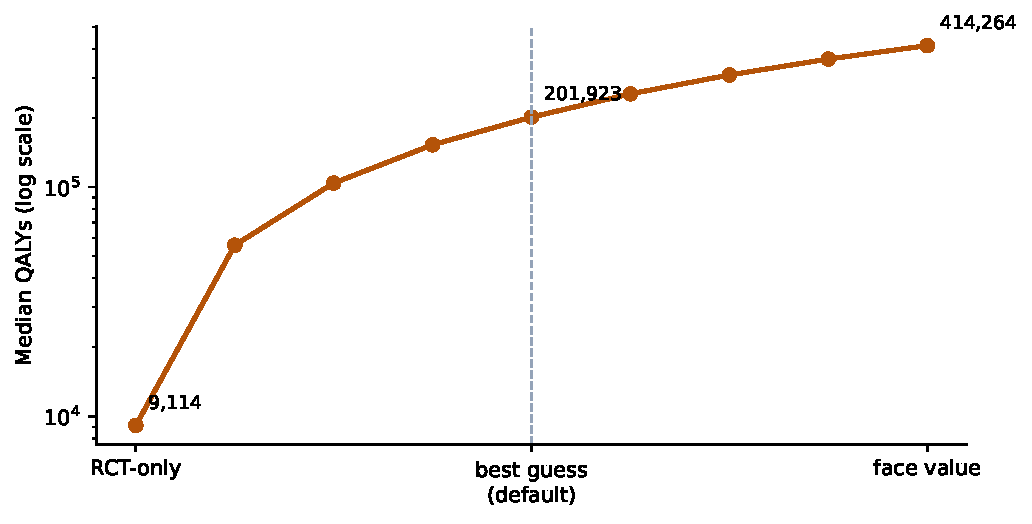
\includegraphics[keepaspectratio]{index_files/figure-pdf/fig-stance-output-1.pdf}}

}

\caption{\label{fig-stance}Median total QALYs across the evidence-stance
range, 100,000 draws per point. The stance interpolates every tier's
credibility mean from an RCT-only floor (non-randomized tiers shrunk to
0.01) through the drafted best-guess tiers (0.5) to face value (1.0).}

\end{figure}%

\textsubscript{Source:
\href{https://MaxGhenis.github.io/mackenzie-scott-qaly/index.qmd.html}{Article
Notebook}}

The dominant sensitivity is not a parameter but a philosophy.
Restricting credit to randomized evidence collapses the median to 9,114
QALYs --- dominated by the one lottery-randomized bucket --- while
taking every cited effect at face value raises it to 414,264
(Figure~\ref{fig-stance}). That 45-fold range dwarfs the spread from any
distributional parameter, and the gap between the face-value and
best-guess estimates is a direct reading of how much of claimed
philanthropic impact rests on evidence that would not survive a
causal-inference seminar. The Spearman tornado
(Figure~\ref{fig-tornado}) tells the same story within the default
stance: the top three drivers are the global-health allocation share,
the realization factor, and global-health credibility.

\begin{figure}

\centering{

\pandocbounded{
\includegraphics[keepaspectratio]{../results/sensitivity.png}}

}

\caption{\label{fig-tornado}What drives the spread: Spearman rank
correlations between each input draw and total QALYs at the best-guess
defaults.}

\end{figure}%

\subsection{The audit moved the headline by less than
2\%}\label{the-audit-moved-the-headline-by-less-than-2}

The geography audit is the largest data correction the model has
absorbed since publication, and its effect is small: recentering the
allocation on audited service geographies moved the abroad share from
4.93\% to 4.82\%, the median from about 205,000 to 201,923, and the
blended figure from about \$148,000 to \$150,067 per QALY. Both
allocations ship with the model, the browser version exposes them as a
version toggle, and the pre-audit parameters remain pinned at tag
\texttt{v2026.07.20} (audited: \texttt{v2026.07.22}).

\subsection{Corrections history}\label{corrections-history}

The model reached this state through eleven public revision rounds, and
the trajectory is itself evidence about the method. Cross-model review
rounds cut the headline from roughly 98,000 to 87,000 QALYs
(dollar-vintage normalization, a life-year/QALY conversion made
explicit, a re-derived frontier benchmark, one re-attributed citation).
Replacing an assumed allocation with the derivation from Scott's own
database cut it to roughly 70,000. A reader's correction --- health
dollars had been priced at U.S. anchors regardless of delivery location
--- tripled it to roughly 205,000, and the subsequent two-model
geography audit settled it at 202,000. Every correction is documented in
the repository and summarized on the public tool; none was caught by the
author unaided, and all but one were caught by models or readers rather
than the author.

\section{Construction and
auditability}\label{construction-and-auditability}

The model was built with a frontier language model (Anthropic's Claude),
with the author reviewing every parameter and assumption; adversarial
review by a second model family (OpenAI's), plus reader corrections,
produced the revision history above. Three mechanisms make the result
checkable rather than merely stated. Parameters live in one typed file
in which every value carries its unit, dollar vintage, and inline
citation, machine-validated at load; an annotated bibliography maps each
quantitative input to its primary source and price-level conversion.
Sync tests force the published web parameters, allocation shares,
geography exports, and this manuscript's inputs to equal fresh
derivations from the committed data snapshots, so prose and model cannot
drift apart. And the audit trail is data: the 990 match audit and the
50-organization geography audit are committed as per-row overlay files
with sources and confidence grades, applied by the pipeline rather than
folded silently into parameters.

The browser implementation is a checked TypeScript port that reruns the
full Monte Carlo client-side; every figure in this paper can be
reproduced, and every assumption overridden, at
\href{https://maxghenis.com/mackenzie-scott-qaly}{maxghenis.com/mackenzie-scott-qaly}.
The repository, including this manuscript's source, is at
\href{https://github.com/MaxGhenis/mackenzie-scott-qaly}{github.com/MaxGhenis/mackenzie-scott-qaly}.

\section{Limitations}\label{limitations}

The credibility tiers and realization distribution are judgment priors
with no literature calibration; the ordering is defensible, the levels
are not measured, and the stance sweep is the honest bound on their
influence. The QALY lens counts only health, so the estimate is a floor
on total wellbeing, and the causes where Scott concentrates ---
education, mobility, equity --- are precisely those whose main benefits
the lens excludes. Credibility shrinks toward zero but never below it,
so the model places no mass on harmful giving. Allocation splits each
organization's dollars equally across its focus areas and service
locations; both are coarse, and the geography audit covers only the 50
largest ``global''-listed organizations. Realization is one global draw,
so it cannot vary by cause. Archetype anchors treat heterogeneous
organizations as draws from one distribution. Within each cause,
delivery regions are priced identically, so the geographic decomposition
exposes assumptions rather than measuring regional differences. The
undisclosed third of dollars is imputed from a fitted elasticity, not
observed. Finally, several anchors rest on a small number of
quasi-experimental papers whose external validity to Scott's grantees is
exactly what the realization factor is guessing at.

\section{Conclusion}\label{conclusion}

Measured in health, MacKenzie Scott's \$26 billion buys a median of
about 202,000 quality-adjusted life-years --- several times its cost at
the government's own valuation --- and most of that health comes from
the twentieth of her dollars delivered in low-income countries. The
number is a model output under stated priors, not a fact, and the
model's most important output is not the point estimate but the
machinery around it: explicit evidence weights, a 45-fold stance range
that any reader can traverse, versioned corrections, and audits
committed as data. Portfolio-scale philanthropy is measurable in
outcomes without waiting for donors to publish outcome data --- their
own gift lists, recipients' tax filings, and the published causal
literature suffice --- and the same machinery applies to any large
giver. The invitation of the interactive version is the paper's real
conclusion: disagree with a parameter, move it, and watch what survives.

\section*{Acknowledgments}\label{acknowledgments}
\addcontentsline{toc}{section}{Acknowledgments}

I thank readers on LinkedIn and the EA Forum whose corrections
materially improved the model, including the reader who identified the
original mispricing of internationally delivered health dollars. The
model, audits, and this manuscript were built with Anthropic's Claude,
with additional adversarial review by OpenAI models; all judgments and
errors are mine. This is a personal research project and does not
represent the views of PolicyEngine or the Axiom Foundation.

\section*{References}\label{references}
\addcontentsline{toc}{section}{References}

\textsubscript{Source:
\href{https://MaxGhenis.github.io/mackenzie-scott-qaly/index.qmd.html}{Article
Notebook}}

\protect\phantomsection\label{refs}
\begin{CSLReferences}{1}{1}
\bibitem[\citeproctext]{ref-bailey2015war}
Bailey, Martha J., and Andrew Goodman-Bacon. 2015. {``The {W}ar on
{P}overty's Experiment in Public Medicine: Community Health Centers and
the Mortality of Older {A}mericans.''} \emph{American Economic Review}
105 (3): 1067--104. \url{https://doi.org/10.1257/aer.20120070}.

\bibitem[\citeproctext]{ref-cep2023gifts}
Center for Effective Philanthropy. 2023. \emph{Emerging Impacts: The
Effects of {M}ac{K}enzie {S}cott's Large, Unrestricted Gifts (Year 2)}.
Center for Effective Philanthropy.
\url{https://cep.org/wp-content/uploads/2023/11/BigGiftsStudy_Report_Y2_FNL.pdf}.

\bibitem[\citeproctext]{ref-cesarini2016wealth}
Cesarini, David, Erik Lindqvist, Robert Östling, and Björn Wallace.
2016. {``Wealth, Health, and Child Development: Evidence from
Administrative Data on {S}wedish Lottery Players.''} \emph{Quarterly
Journal of Economics} 131 (2): 687--738.
\url{https://doi.org/10.1093/qje/qjw001}.

\bibitem[\citeproctext]{ref-givewell2024cash}
GiveWell. 2024. \emph{Re-Evaluating the Impact of Unconditional Cash
Transfers}.
\href{https://blog.givewell.org/2024/11/12/re-evaluating-the-impact-of-unconditional-cash-transfers/}{Https://blog.givewell.org/2024/11/12/re-evaluating-the-impact-of-unconditional-cash-transfers/}.

\bibitem[\citeproctext]{ref-givewell2026impact}
GiveWell. 2026. \emph{Impact Estimates}.
\href{https://www.givewell.org/impact-estimates}{Https://www.givewell.org/impact-estimates}.

\bibitem[\citeproctext]{ref-givingusa2026}
Indiana University Lilly Family School of Philanthropy. 2026.
\emph{Giving {USA} 2026: The Annual Report on Philanthropy for the Year
2025}. Giving USA Foundation.

\bibitem[\citeproctext]{ref-cnbc2025scott}
Konish, Lorie. 2025. \emph{{M}ac{K}enzie {S}cott Revealed Her Total
Charitable Donations for 2025}.
\href{https://www.cnbc.com/2025/12/13/mackenzie-scott-revealed-her-total-charitable-donations-for-2025.html}{Https://www.cnbc.com/2025/12/13/mackenzie-scott-revealed-her-total-charitable-donations-for-2025.html}.

\bibitem[\citeproctext]{ref-miller2021medicaid}
Miller, Sarah, Norman Johnson, and Laura R. Wherry. 2021. {``Medicaid
and Mortality: New Evidence from Linked Survey and Administrative
Data.''} \emph{Quarterly Journal of Economics} 136 (3): 1783--829.
\url{https://doi.org/10.1093/qje/qjab004}.

\bibitem[\citeproctext]{ref-propublica2026}
ProPublica. 2026. \emph{Nonprofit Explorer}.
\href{https://projects.propublica.org/nonprofits/}{Https://projects.propublica.org/nonprofits/}.

\bibitem[\citeproctext]{ref-sommers2017medicaid}
Sommers, Benjamin D. 2017. {``State {M}edicaid Expansions and Mortality,
Revisited: A Cost-Benefit Analysis.''} \emph{American Journal of Health
Economics} 3 (3): 392--421. \url{https://doi.org/10.1162/ajhe_a_00080}.

\bibitem[\citeproctext]{ref-aspe2026values}
U.S. Department of Health and Human Services, Office of the Assistant
Secretary for Planning and Evaluation. 2026. \emph{Standard Values for
Regulatory Impact Analysis}. ASPE.
\url{https://aspe.hhs.gov/reports/standard-ria-values}.

\bibitem[\citeproctext]{ref-yieldgiving2026}
Yield Giving. 2026. \emph{Gifts Database}.
\href{https://yieldgiving.com/gifts}{Https://yieldgiving.com/gifts}.

\end{CSLReferences}




\end{document}
